\chapter{Static Analysis}

L'obiettivo di questa challenge (proposta dal GitHub Security Lab) è testare e migliorare le abilità di \textit{vulnerability hunting} imparando a padroneggiare CodeQL. La missione consiste nel trovare le \textbf{13 vulnerabilità critiche di Remote Code Execution (RCE)} scoperte dai ricercatori all'interno del bootloader \textbf{U-Boot}. Queste vulnerabilità (identificate dai CVE da CVE-2019-14192 a CVE-2019-14204) si innescano quando U-Boot è configurato per utilizzare la connessione di rete al fine di eseguire il fetching delle risorse di avvio. Il problema di fondo è un potenziale \textbf{buffer overflow} controllato dall'attaccante.

Per individuare i bug in modo mirato, la soluzione CodeQL è stata costruita mediante un approccio step-by-step, imparando gradualmente come modellare le chiamate del codice C e filtrando man mano le chiamate non sicure, fino ad arrivare al file decisivo \texttt{10\_taint\_tracking.ql} in cui viene formalizzata l'analisi finale.

\section{Il Risultato della Query (\texttt{10\_taint\_tracking.ql})}

La query finale costruita nel decimo step è un'analisi automatica volta a tracciare in modo accurato se i valori provenienti dall'esterno finiscono in chiamate insicure della funzione \texttt{memcpy}. 
Nello specifico, utilizzando la libreria \texttt{TaintTracking} di CodeQL (un'analisi \textbf{path-problem} che mostra visivamente in GitHub il percorso dai dati compromessi all'uso), la query rileva casi in cui:
\begin{itemize}
  \item \textbf{La Sorgente (Source):} Un dato in ingresso controllato dall'attaccante proviene dal network (delineato dai risultati delle macro di conversione byte come \texttt{ntohs}, \texttt{ntohl}, \texttt{ntohll}).
  \item \textbf{Il Pozzo (Sink):} Questo dato finisce direttamente per essere utilizzato come argomento della ``dimensione'' parametrizzata in una chiamata \texttt{memcpy}, indicata tramite \texttt{call.getArgument(2)} nel codice.
\end{itemize}

Se la query traccia con successo l'intero percorso dalla \textit{Sorgente} al \textit{Sink}, solleverà un avviso identificando la fetta di codice fallata e mostrando l'errore: \textit{``Network byte swap flows to memcpy without validation''}.

\begin{figure}[H]
  \centering
  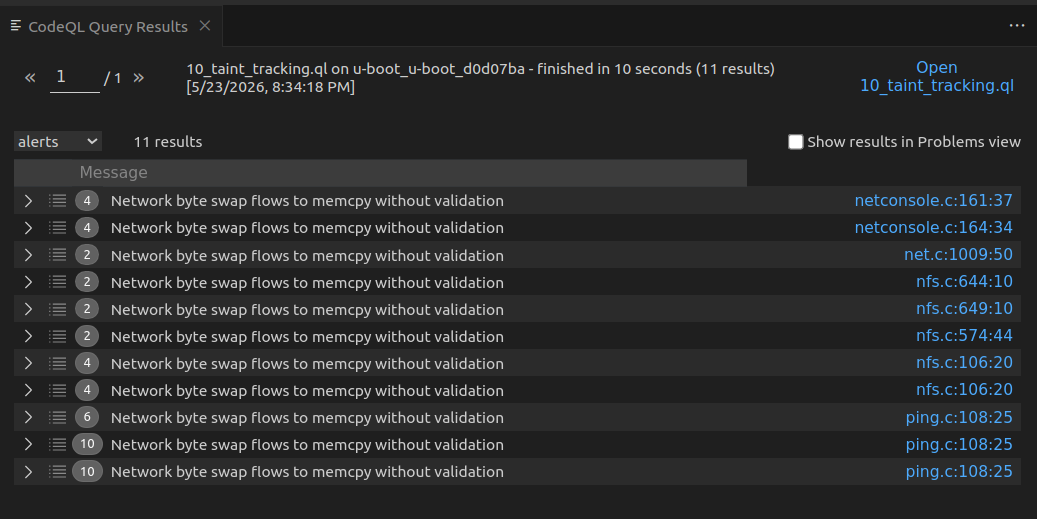
\includegraphics[width=0.7\textwidth]{../4.StaticAnalysis/img/Query_result.png}
  \caption{Risultato della query su GitHub}
\end{figure}

\section{Il predicato \texttt{isBarrier} per la sanificazione}

Durante la costruzione dell'analisi, sorgono facilmente dei \textit{falsi positivi}: cosa succede se lo sviluppatore utilizza i dati in ingresso e chiama la \texttt{memcpy}, ma prima effettua un controllo sicuro imponendo limiti massimi di grandezza? 
In questi casi il flusso deve interrompersi per validare l'assenza di vulnerabilità. Questo è compito del predicato \texttt{isBarrier(DataFlow::Node node)}:
\begin{enumerate}
  \item \textbf{Controlla un blocco relazionale:} Identifica l'esistenza di una condizione di guardia (es. uno statement \texttt{if}) determinata da operatori relazionali (come \texttt{<}, \texttt{>}, \texttt{<=}, \texttt{>=}).
  \item \textbf{Identifica il campo d'azione:} Si assicura che il nodo che CodeQL sta scansionando (la variabile \texttt{v} \textit{tainted}) stia venendo richiamato.
  \item \textbf{Verifica il limite (Bound check):} Constata che a essere verificata da quell'operatore logico/relazionale sia esattamente quella variabile (se si trova a destra o a sinistra dell'operazione, come ad es. \texttt{length < MAX\_SIZE}).
  \item \textbf{Isola la via sicura:} Conferma infine che questa guardia tuteli il Basic Block esecutivo nel suo ramo \texttt{true}; cioè, l'esecuzione approderà al nodo in cui risiede la \textit{Sink} (la potenziale \texttt{memcpy}) unicamente se l'esito della validazione di sicurezza darà esito positivo. In tal modo erige la ``barriera'', bloccando CodeQL dal segnalarlo come minaccia tra gli eventi di sicurezza.
\end{enumerate}

\section{Automazione con GitHub Actions (\texttt{main.yml})}

Oltre alla validazione e stesura locale della query, è stato integrato un workflow GitHub Actions in \texttt{.github/workflows/main.yml} per un'individuazione trasparente sul repository, simulando un vero applicativo SAST. 

I passaggi principali operati dal virtual environment Ubuntu garantiscono:
\begin{itemize}
  \item \textbf{Trigger event:} Si aziona a ogni singola \texttt{push} direttamente sul branch \texttt{main} (o tramite procedura manuale \textit{dispatch}).
  \item \textbf{Checkout \& Environment:} Preleva il codice sorgente e inizializza l'azione nativa \texttt{github/codeql-action/init@v3} per analizzare il linguaggio C/C++ (\texttt{cpp}), dicendo a CodeQL di focalizzarsi unicamente sulla custom query finale prodotta (\texttt{./4.StaticAnalysis/query\_github\_actions/10\_taint\_tracking.ql}).
  \item \textbf{Dependency Install \& Intercepting Build:} Essendo un linguaggio compilato, CodeQL richiede di ``ascoltare e tracciare'' l'intera procedura di build del progetto per costruirsi a ritroso il database semantico del codice del progetto. A questo scopo, il workflow installa dipendenze chiave per l'utility, entra nel modulo \texttt{u-boot}, lo configura con \texttt{make sandbox\_defconfig} (creando un'infrastruttura di test) per poi iniziare un massiccio processo di make tracciato.
  \item \textbf{Reporting:} Come step finale, scatta \texttt{analyze@v3}. CodeQL sfrutta il database generatosi per eseguire la problem-query, postando gli avvisi localizzati e visibili all'interno della dashboard Security > Code scanning sulla repository di GitHub.
\end{itemize}